\subsection{マップ・詳細画面}
マップ・詳細画面ではカードリスト画面でユーザがタップしたカードに対応するスポットの場所をピンとしてマップ中央に表示する。また、カードリスト画面でユーザがお気に入りとして星をつけた場合は対応するスポットの場所を星としてマップ上に表示する。ピン又は星をタップするたびに画面下に表示しているカード情報が対応するスポットの内容に変わる仕様である。通常、画面下のカード情報はお店の営業時間や有名商品の値段などを表示しているが、右向きの矢印をタップすることでカードリスト画面にも表示しているスポットの紹介文へと表示内容が切り替わる。スポットの紹介文を表示中は左向きの矢印となり、それをタップすることで通常の詳細情報の表示へと切り替わる。マップ・詳細画面で使用したアイコンの意味については表6.2を参照されたい。

\begin{table}[htb]
\centering
\addtocounter{table}{+1}
\caption{アイコン一覧と意味}
  \begin{tabular}{|c|c|} \hline
    アイコン&意味  \\ \hline 
    \begin{minipage}{10mm}
      \centering
      \scalebox{0.4}{
\includegraphics{redpin.png}}
    \end{minipage} & \parbox{38zw}{Google Mapsで使用されておりユーザにピンということを伝えるためにこのアイコンを使用した} \\  \hline
    \begin{minipage}{10mm}
      \centering
      \scalebox{0.3}{
\includegraphics{favourites.png}}
    \end{minipage} &\parbox{38zw}{Twitterで長年使用されていた星がお気に入りの印象付けが根強いと判断し使用した}\\ \hline
     \begin{minipage}{10mm}
      \centering
      \scalebox{0.5}{
\includegraphics{arrow.png}}
    \end{minipage} & \parbox{38zw}{右側又は左側に何かあるということを伝達するために矢印を使用した}\\ \hline
  \end{tabular} 
\end{table}

\addtocounter{figure}{+1}
\begin{figure}[htbp]
  \begin{center}
    \begin{tabular}{c}

      % 1
      \begin{minipage}{0.33\hsize}
        \begin{center}
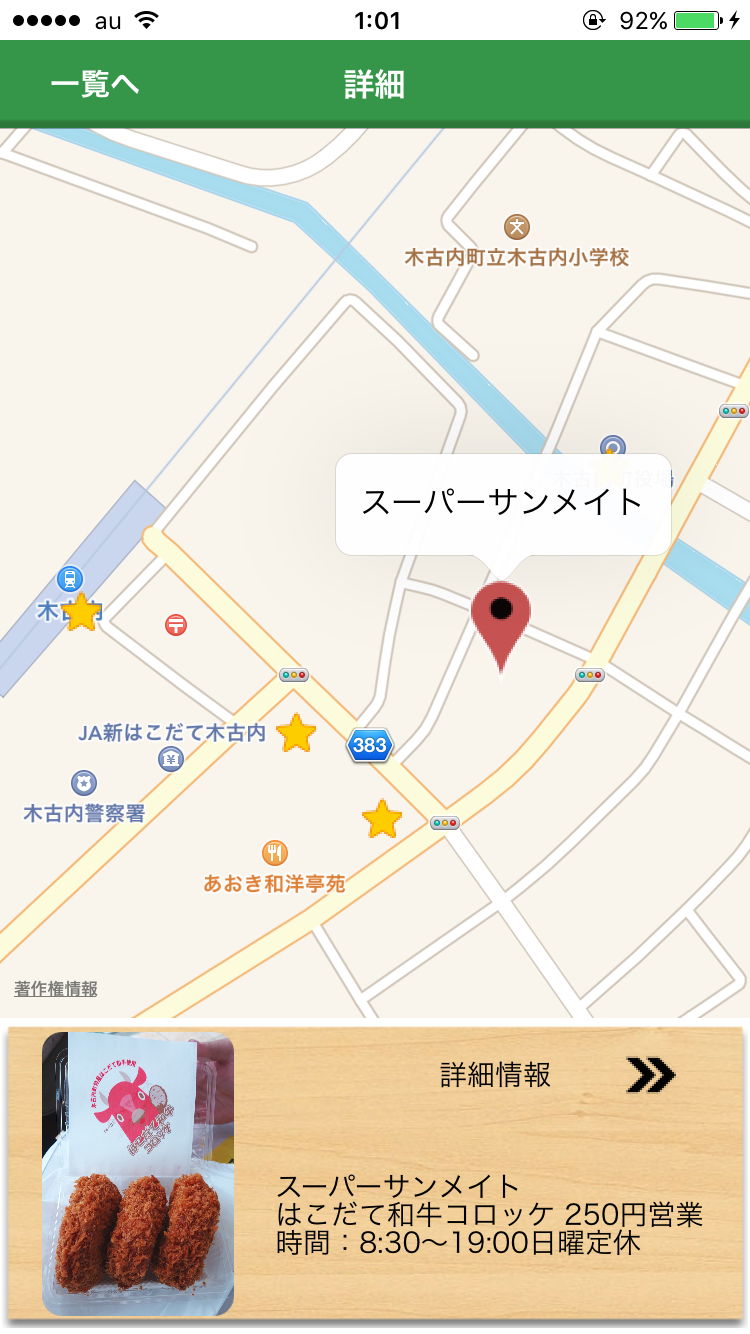
\includegraphics[width=4cm, bb=0 0 303 573]{kiko_map1.png}
          \hspace{1cm} (a)詳細情報表示中
        \end{center}
      \end{minipage}

      % 2
      \begin{minipage}{0.33\hsize}
        \begin{center}
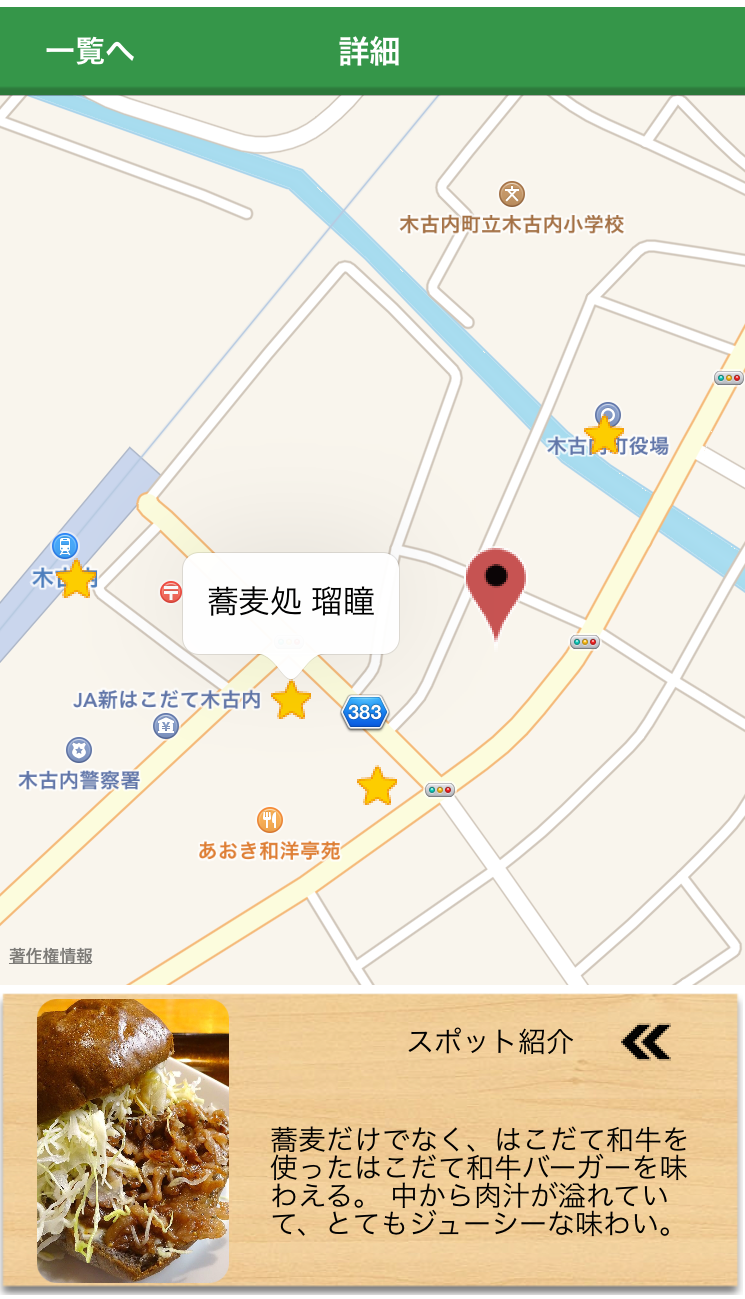
\includegraphics[width=4cm, bb=0 0 304 570]{kiko_map2.png}
          \hspace{1cm} (b)スポット紹介表示中
        \end{center}
      \end{minipage}

    \end{tabular}
    \caption{マップ・詳細画面}
    \label{fig:lena}
  \end{center}
\end{figure}
\bunseki{岩見建汰}